\documentclass{article}
\newcommand{\BEAS}{\begin{eqnarray*}}
\newcommand{\EEAS}{\end{eqnarray*}}
\newcommand{\BEQ}{\begin{equation}}
\newcommand{\EEQ}{\end{equation}}
\newcommand{\BIT}{\begin{itemize}}
\newcommand{\EIT}{\end{itemize}}

\newcommand{\eg}{{\it e.g.\ }}
\newcommand{\ie}{{\it i.e.\ }}

\newcommand{\ones}{\mathbf 1}
\newcommand{\zeros}{\mathbf 0}
\newcommand{\reals}{{\mbox{\bf R}}}
\newcommand{\integers}{{\mbox{\bf Z}}}
\newcommand{\symm}{{\mbox{\bf S}}}  % symmetric matrices

\newcommand{\nullspace}{{\mathcal N}}
\newcommand{\range}{{\mathcal R}}
\newcommand{\Rank}{\mathop{\bf Rank}}
\newcommand{\Tr}{\mathop{\bf Tr}}

\newcommand{\sign}[1]{\mathop{\textrm{sgn}}(#1)}
\newcommand{\lambdamax}{{\lambda_{\rm max}}}
\newcommand{\lambdamin}{\lambda_{\rm min}}

\newcommand{\EE}{\mathop{\textrm{E}}}
\newcommand{\Cov}{\mathop{\textrm{Cov}}}
\newcommand{\Prob}{\mathop{\bf Prob}}
\newcommand{\Co}{{\mathop {\bf Co}}} % convex hull
\newcommand{\dist}{\mathop{\bf dist{}}}
\newcommand{\argmin}{\mathop{\rm argmin}}
\newcommand{\argmax}{\mathop{\rm argmax}}
\newcommand{\epi}{\mathop{\bf epi}} % epigraph
\newcommand{\Vol}{\mathop{\bf vol}}
\newcommand{\dom}{\mathop{\bf dom}} % domain
\newcommand{\intr}{\mathop{\bf int}}


\newcommand{\nrm}[1]{\left\lVert#1\right\rVert}
\newcommand{\nrmo}[1]{\left\lVert#1\right\rVert_1}
\newcommand{\nrmt}[1]{\left\lVert#1\right\rVert_2}
\newcommand{\nrmnn}[1]{\left\lVert#1\right\rVert_{*}}
\newcommand{\nrmf}[1]{\left\lVert#1\right\rVert_F}

\newcommand{\myexp}[1]{\mathop{\rm exp}\left\{#1\right\}}
\newcommand{\mylog}[1]{\mathop{\rm log}\left\{#1\right\}}
\newcommand{\questions}{\begin{frame}Questions?\end{frame}}
\newcommand{\LL}{\textrm{LL}}
\newcommand{\KL}{\textrm{KL}}
\newcommand{\HH}{\textrm{H}}
\newcommand{\GG}{\textrm{G}}

\newcommand{\Bound}{\textrm{B}}
\newcommand{\bb}{\mathbf{b}}
\newcommand{\aaa}{\mathbf{a}}
\newcommand{\BB}{\mathbf{B}}
\newcommand{\AAA}{\mathbf{A}}
\newcommand{\CC}{\mathbf{C}}
\newcommand{\cc}{\mathbf{c}}
\newcommand{\mm}{\mathbf{m}}
\newcommand{\MM}{\mathbf{M}}
\newcommand{\nn}{\mathrm{\bf neighbors}}
\newcommand{\pa}[1]{{\textrm{\bf pa}}\left(#1\right)}
\newcommand{\pre}[2]{\mathop{\textrm{\bf pnp}}_{#1}\left(#2\right)}
\newcommand{\logsum}{\textrm{logsum}}

\newcommand{\tth}{{\textrm{th}}}
\newcommand{\xx}{\mathbf{x}}
\newcommand{\mmu}{\mathbf{\mu}}
\newcommand{\yy}{\mathbf{y}}
\newcommand{\zz}{\mathbf{z}}
\newcommand{\dd}{\mathbf{d}}
\newcommand{\new}{\textrm{new}}
\newcommand{\old}{\textrm{old}}
\newcommand{\fpr}{\textrm{FPR}}
\newcommand{\tpr}{\textrm{TPR}}
\newcommand{\auc}{\textrm{AUC}}
\newcommand{\yyi}{\yy_i}
\newcommand{\xxi}{\xx_i}
\newcommand{\vvec}[2]{\left[ \begin{array}{c} \mathbf{#1}\\ \mathbf{#2} \end{array}\right]}
\newcommand{\mmat}[4]{\left[ \begin{array}{cc} \mathbf{#1}&\mathbf{#2}\\ \mathbf{#3}&\mathbf{#4} \end{array}\right]}
\newcommand{\xyvec}{\left[ \begin{array}{c} \xx\\\yy \end{array} \right]}
\newcommand{\xyvecc}{\left[ \begin{array}{c} x^1\\y^1 \end{array} \right]}
\newcommand{\eye}{   \left[ \begin{array}{cc} 1 & 0 \\ 0 & 1 \end{array}\right]}
\newcommand{\bket}[2]{\left\langle#1,#2\right\rangle}
\newcommand{\bbket}[2]{\left\llangle#1,#2\right\rrangle}
\newcommand{\redq}{\textcolor{red}{q}}
\newcommand{\blup}{\textcolor{blue}{p}}
\newcommand{\BIEA}{\begin{IEEEeqnarray*}}
\newcommand{\EIEA}{\end{IEEEeqnarray*}}
\newcommand{\BIEAN}{\begin{IEEEeqnarray}}
\newcommand{\EIEAN}{\end{IEEEeqnarray}}
\newcommand{\pmin}{\mathop{\textrm{minimize}}}
\newcommand{\psubjto}{\textrm{subject to}}
\newcommand{\WW}{\mathbf{W}}
\newcommand{\ww}{\mathbf{w}}
\newcommand{\YY}{\mathbf{Y}}
\newcommand{\XX}{\mathbf{X}}
\newcommand{\UU}{\mathbf{U}}
\newcommand{\uu}{\mathbf{u}}
\newcommand{\VV}{\mathbf{V}}
\newcommand{\vv}{\mathbf{v}}
\newcommand{\PP}{\mathbf{P}}
\newcommand{\pp}{\mathbf{p}}
\newcommand{\rr}{\mathbf{r}}
\newcommand{\RR}{\mathbf{R}}
\newcommand{\ee}{\mathbf{e}}
\newcommand{\II}{\mathbf{I}}
\newcommand{\DD}{\mathbf{D}}

\newcommand{\aalpha}{{\boldsymbol\alpha}}
\newcommand{\llambda}{{\boldsymbol\lambda}}
\newcommand{\ddelta}{{\boldsymbol\delta}}
\newcommand{\otherwise}{\textrm{otherwise}}
\newcommand{\answer}{\fbox{\tt answer} }
\newcommand{\abs}[1]{\left| #1 \right|}

\newcounter{problemCtr}
\newcommand{\newproblem}[1]{\hrule\paragraph{Problem \theproblemCtr (#1)}\stepcounter{problemCtr}}


\newcounter{HW}

\usepackage{amsthm}
\usepackage{graphicx}
\usepackage{natbib}
\usepackage{algorithm}
\usepackage{algorithmic}
\usepackage{amsmath}
\usepackage{hyperref}
\usepackage{tikz}


\newtheorem{remark}{Remark}
\newtheorem{lemma}{Lemma}
\newtheorem{definition}{Definition}
\newtheorem{proposition}{Proposition}
\newtheorem{assumption}{Assumption}
\newtheorem{corollary}{Corollary}
\newtheorem{theorem}{Theorem}


\begin{document}
\author{Ravikiran Janardhana}
\setcounter{HW}{2}
\title{COMP  790-124, HW\theHW}
\maketitle


{ Deadline: 10/24/2012 11:59PM EST}

{ Submit \texttt{hw\theHW.pdf} by e-mail to \texttt{vjojic+comp790+hw\theHW@cs.unc.edu}



\noindent\rule{\textwidth}{3pt}


In the next few problems we will derive and implement an ADMM algorithm for logistic regression with a fused lasso penalty.  You can refer to the ADMM write up available on the course website  \url{http://www.cs.unc.edu/~vjojic/comp790/notes/ADMMFLSA.pdf}, but note that, while there are similarities with the problems below, there are differences as well.

\newproblem{1pt}
The optimization problem for logistic regression with a fused lasso penalty is given as
\BEAS
\mathop{\textrm{minimize}}_{\ww} && \sum_i \mylog{1 + \myexp{-y_i(\xx_i\ww)}} + \\
&&\lambda\nrmo{\ww} + \mu\nrmo{\DD\ww}.
\EEAS
We are going to introduce new variables $\zz^0, \zz^1, \zz^2$ and reformulate the problem
\BEAS
\mathop{\textrm{minimize}}_{\ww,\zz_0,\zz_1,\zz^2} && \sum_i \mylog{1 + \myexp{-y_i\zz^0}} + \lambda\nrmo{\zz^1} + \mu\nrmo{\zz^2}\\
\textrm{subject to} && z^0_i = \xx_i\ww, i=1,\dots n \\
&& \zz^1 = \ww \\
&& \zz^2 = \DD\ww
\EEAS

Write out the augmented lagrangian for the above problem
\BEAS
\textrm{AL}(\ww,\zz^0,\zz^1,\zz^2,\uu^0,\uu^1,\uu^2) &=&  \sum_i \log\{1+\exp\{-y_{i}z_{i}^{0}\}\} + \lambda\nrmo{\zz^{1}} + \mu\nrmo{\zz^2} + \\
&& \sum_{i} u_{i}^{0} (z_{i}^{0} - \xx_{i}\ww) + \uu^{1} (\zz^{1} - \ww) + \uu^{2} (\zz^{2} - \DD\ww) + \\
&& \sum_{i} \frac{\rho}{2} \nrmt{z_{i}^{0} - \xx_{i}\ww}^{2} + \frac{\rho}{2} \nrmt{\zz^{1} - \ww}^{2} + \frac{\rho}{2} \nrmt{\zz^{2} - \DD\ww}^{2} \\
\EEAS

Hint: Make sure that you have all the terms from the objective, that is logistic regression and the two norms. For each constraint you should have a term that involves the dual variables, for example $u^0_i(z^0_i - \xx_i\ww)$, and a term that augments the lagrangian, for example $\frac{\rho}{2}\nrmt{z^0_i - \xx_i\ww}$.

\newproblem{1pt}
Implement function that computes the value of augmented lagrangian
\begin{verbatim}
function val = computeAL(y, X, D, lambda, mu, rho, w, z0, z1, z2, u0, u1, u2)
    term11 = 0.0;
    for i = 1 : size(y, 2)
        term11 = term11 + log(1 + exp(-1 .* y(i) .* z0(i)));
    end
    term12 = lambda * computeL1Norm(z1);
    term13 = mu * computeL1Norm(z2);
    
    term21 = 0.0;
    for i = 1 : size(z0, 2)
        term21 = term21 + (u0(i) * (z0(i) - w * X(:,i)));
    end
    term22 = u1 * (z1 - w);
    term23 = u2 * (z2 - w * D);
    
    term31 = 0.0;
    for i = 1 : size(z, 2)
        term31 = term21 + ((rho/2) * computeL2Norm(z0(i) - (w * X(:, i))).^2);        
    end
    term32 = (rho/2) * (computeL2Norm(z1 - w).^2);
    term33 = (rho/2) * (computeL2Norm(z2 - w * D).^2);
    
    val = term11 + term12 + term13 + ...
          term21 + term22 + term23 + ...
          term31 + term32 + term33;
end

function value = computeL1Norm(z)
    value = 0;
    for i = 1 : size(z, 2)
        value = value + abs(z(i));
    end
end

function value = computeL2Norm(z)
    value = 0;
    for i = 1 : size(z, 2)
        value = value + abs(z(i)).^2;
    end
    value = sqrt(value);
end
\end{verbatim}


\newproblem{1pt}
We will use superscript $k$ to indicate the iteration, so for example $\ww^k$ denotes the state of variable $\ww$ in the $k^\tth$ iteration. Collect the terms in the augmented lagrangian that involve $\ww$, complete the square and plug in the resulting expression below
\BEAS
\ww^k &=& \argmin_\ww \sum_{i} u_{i}^{0,k-1} (z_{i}^{0,k-1} - \xx_{i}\ww) + \uu^{1,k-1} (\zz^{1,k-1} - \ww) + \uu^{2} (\zz^{2,k-1} - \DD\ww) + \\
&& \sum_{i} \frac{\rho}{2} \nrmt{z_{i}^{0,k-1} - \xx_{i}\ww}^{2} + \frac{\rho}{2} \nrmt{\zz^{1,k-1} - \ww}^{2} + \frac{\rho}{2} \nrmt{\zz^{2,k-1} - \DD\ww}^{2} 
\EEAS

\BEAS
\ww^k &=& \argmin_\ww \sum_{i} \frac{\rho}{2} \nrmt{z_{i}^{0,k-1} - \xx_{i}\ww + \frac{1}{\rho}u_{i}^{0,k-1}}^{2} + \\
&& \frac{\rho}{2} \nrmt{z^{1,k-1} - \ww + \frac{1}{\rho}\uu^{1,k-1}}^{2} + \\
&& \frac{\rho}{2} \nrmt{z^{2,k-1} - \DD\ww + \frac{1}{\rho}\uu^{2,k-1}}^{2} 
\EEAS

\BEAS
\ww^k &=& \argmin_\ww \frac{\rho}{2} \nrmt{\begin{bmatrix} \xx \\ \II \\ \DD \end{bmatrix}\ww - \begin{bmatrix} \zz^{0,k-1} + \frac{1}{\rho} \uu^{0, k-1} \\ \zz^{1,k-1} + \frac{1}{\rho} \uu^{1, k-1} \\ \zz^{2,k-1} + \frac{1}{\rho} \uu^{2, k-1} \end{bmatrix} }^{2} 
\EEAS

When completing squares here do it so that $\ww,\uu_0,\zz_0$ occur under one, $\ww,\uu_1,\zz_1$ occur under another, and $\ww,\uu_1,\zz_2$ occur under yet another norm term.

Same thing for $z^0_i$, note that here we are considering just a single $z^0_i$ not the full vector. You can convince yourself that if you write out the objective for the full vector it is separable into objectives across $z^0_i$.
\BEAS
z_i^{0,k} &=& \argmin_{z_i^0}   \log{\{1+exp\{-y_{i}z_{i}^{0}\}\}} + \frac{\rho}{2}\nrmt{z_{i}^{0}-\xx_{i}\ww^{k}+\frac{1}{\rho}u_{i}^{0,k-1}}^{2} 
\EEAS
And once more for $z^1_i$, using the fact that $\nrmo{\zz^1} = \sum_i |z^1_i|$
\BEAS
z_i^{1,k} &=& \argmin_{z_i^1}   \frac{\lambda}{\rho}\nrmo{z_{i}^{1}} + \frac{1}{2} \nrmt{z_{i}^{1} - \ww^{k} + \frac{1}{\rho}u_{i}^{1,k-1}}^{2} 
\EEAS
Finally, do the same for $z^2_i$
\BEAS
z_i^{2,k} &=& \argmin_{z_i^2}   \frac{\mu}{\rho} \nrmo{z_{i}^{2}} + \frac{1}{2} \nrmt{z_{i}^{2} - \DD\ww^{k} + \frac{1}{\rho}u_{i}^{2,k-1}}^{2} 
\EEAS


\newproblem{1pt} Copy over the update for $\ww$ from above
\BEAS
\ww^k &=& \argmin_\ww  \frac{\rho}{2} \nrmt{\begin{bmatrix} \xx \\ \II \\ \DD \end{bmatrix}\ww - \begin{bmatrix} \zz^{0,k-1} + \frac{1}{\rho} \uu^{0, k-1} \\ \zz^{1,k-1} + \frac{1}{\rho} \uu^{1, k-1} \\ \zz^{2,k-1} + \frac{1}{\rho} \uu^{2, k-1} \end{bmatrix} }^{2}
\EEAS
Note that $\ww = \II\ww$ and refer to the appendix of the Lecture 4 notes on how to stack these two linear systems, as well as code to do it. Of course, the ADMM writeup also has some of this. Implement a function that gives update for $\ww$
\begin{verbatim}
function  w  =  updatew(X, n, D, z0, z1, z2, u0, u1, u2, rho)
    w  =  [X; eye(n); D] \ [z0+((1/rho)*u0); z1+((1/rho)*u1); z2+((1/rho)*u2)];
end
\end{verbatim}

\newproblem{1pt}
To update $z^0_i$ we will be solving an optimization problem
\[
\mathop{\textrm{minimize}}_{z \in \reals} \mylog{1 + \myexp{-yz}} + \gamma(z - a)^2.
\]
Note that $z$ is a scalar, so the objective is univariate.
Here is a an implementation of Newton algorithm with backtracking, it takes a function handle and starting value as a input.


\begin{verbatim}
function z = newtonWolfeBacktrack(objective, initZ)
% newtonWolfeBacktrack solves an unconstrained optimization problem
%    using Newton's method with backtracking and the Weak Wolfe
%    condition for backtracking termination.
%
% z = newtonWolfeBacktrack(objective, initZ)
%   objective  a handle of function that take input z and returns
%              the values of the objective, the first, and the
%              second derivative at z
%   initZ      initial value of z
%
ALPHA = 0.05;
BETA = 0.5;
TOL = 1e-6;
MAX_ITER = 100;
z = initZ;
for it=1:MAX_ITER
    [val,d,dd] = objective(z);

    % Newton direction
    dz = -d/dd;

    % we are done if derivative is small enough
    if abs(dz) < TOL
        break;
    end

    % backtracking with the Wolfe condition check
    step = 1;
    while objective(z + step*dz) > val + ALPHA*step*dz*d
          step = step*BETA;
    end
    z = z + step*dz;
end
\end{verbatim}
Save this file as \texttt{newtonWolfeBacktrack.m}. In the code above, the while loop is terminated when the Wolfe condition is satisfied. Read the code and explain what the Wolfe condition is trying to accomplish. 

\textbf{Ans.} The Wolfe condition is trying to reduce the \textbf{step}(step length) by BETA = 0.5 at each iteration such that the objective(z + step*z) is less than (objective(z) + ALPHA * step * dz * d).

This is nothing but the sufficient decrease condition for minimizing the objective function and we break out of the while loop when the above condition is satisfied.

Now we will write a function that computes the objective and its derivatives.
\begin{verbatim}
function  [val,d,dd]  =  logRegGaussPrior(z,y,a,gamma)
    val  =  log(1  +  exp(-y*z))  +  gamma*(z-a)^2;
    if  nargout  >  1  %  caller  asked  for  derivatives
        d = (-y ./ (1 + exp(y*z))) + (2 * gamma * (z - a));
        dd = ((y.^2 * exp(y*z)) ./ ((1 + exp(y*z)).^2)) + (2 * gamma);  
    end
end
\end{verbatim}

An example of how to use these two pieces together:
\begin{verbatim}
y = 1; a = 0.1; gamma = 0.5;
f = @(z) logRegGaussPrior(z,y,a,gamma);
z = newtonWolfeBacktrack(f,0);
\end{verbatim}
Of course you will be plugging in different values of \texttt{y,a,gamma}. Note that \texttt{f} is really a function with some arguments to \texttt{logRegGaussPrior} hardcoded. In the above example \texttt{0.1} will be hardcoded in the definition of \texttt{f}.  So even if you subsequently change variable \texttt{a}, the function \texttt{f} will still supply \texttt{0.1} as the third argument to \texttt{logRegGaussPrior}.

Use the \texttt{newtonWolfeBacktrack} and \texttt{logRegGaussianPrior} to implement
\begin{verbatim}
function z0i = updatez0i(yi, xi, w, u0i, rho)
    y = yi;    
    a = (xi*w) - ((1/rho) * u0i);
    gamma = rho/2;
    f = @(z) logRegGaussPrior(z,y,a,gamma);
    z0i = newtonWolfeBacktrack(f,0);    
end
\end{verbatim}

\newproblem{1pt} Copy over update for $z^1$ from above
\[
z_i^{1,k} = \argmin_{z_I^1}   \frac{\lambda}{\rho}\nrmo{z_{i}^{1}} + \frac{1}{2} \nrmt{z_{i}^{1} - \ww^{k} + \frac{1}{\rho}u_{i}^{1,k-1}}^{2}
\]

Refer to ADMM writeup on how to solve this in a closed form the problem of this shape and write it out here.

The optimization is simply Lasso regression and can be solved in a closed form update as below (where S is shrinkThreshold function and is implemented as below):-
\[
z_i^{1,k} = S(\ww^{k} - \frac{1}{\rho}u_{i}^{1,k-1}, \frac{\lambda}{\rho}) 
\]
write code to implement this update
\begin{verbatim}
function z1i = updatez1i(w, u1i, lambda, rho)
    z1i = shrinkThreshold(w - 1/rho*u1i, lambda/rho);        
end

function  x  =  shrinkThreshold(x,lambda)
    x  =  sign(x).*max(abs(x)  -  lambda,0);
end
\end{verbatim}


\newproblem{1pt} Copy over update for $z_i^2$ from above
\[
z_i^{2,k} = \argmin_{z_i^2}   \frac{\mu}{\rho} \nrmo{z_{i}^{2}} + \frac{1}{2} \nrmt{z_{i}^{2} - \DD\ww^{k} + \frac{1}{\rho}u_{i}^{2,k-1}}^{2} 
\]

Refer to ADMM writeup on how to solve this in a closed form the problem of this shape and write it out here.

The optimization is simply Lasso regression and can be solved in a closed form update as below (where S is shrinkThreshold function and is implemented as below):-
\[
z_i^{2,k} = S(\DD\ww^{k} - \frac{1}{\rho}u_{i}^{2, k-1}, \frac{\mu}{\rho}) 
\]
write code to implement this update
\begin{verbatim}
% Dwi = Dw(i), Dw = D*w
function z2i = updatez2i(Dwi, u2i, mu, rho)    
    z2i = shrinkThreshold(Dwi - 1/rho*u2i, mu/rho);
end

function  x  =  shrinkThreshold(x,lambda)
    x  =  sign(x).*max(abs(x)  -  lambda,0);
end
\end{verbatim}

\newproblem{2pt} Putting all of this together
\begin{verbatim}
function  w  =  solveLogRegFusedLasso(y,X,D, lambda, mu)
    rho  =  1;
    N  =  length(y);  assert(N  ==  size(X,1));
    p  =  size(X,2);  assert(p  ==  size(D,2));
    e  =  size(D,1);
    w  =  zeros(p,1);
    z0  =  zeros(N,1);  u0  =  zeros(N,1);
    z1  =  zeros(p,1);  u1  =  zeros(p,1);
    z2  =  zeros(e,1);  u2  =  zeros(e,1);
    MAXIT  =  100;
    n = size(X, 2);
    
    for  it=1:MAXIT
        before  =  computeAL(y,X,D,lambda,mu,rho,w,z0,z1,z2,u0,u1,u2);        
        w = updatew(X, n, D, z0, z1, z2, u0, u1, u2, rho);
        after  =  computeAL(y,X,D,lambda,mu,rho,w,z0,z1,z2,u0,u1,u2);
        assert(after  <  before  +  1e-6);
        
        before  =  after;
        for  i=1:length(y)
            z0(i)  =  updatez0i(y(i), X(i,:), w, u0(i), rho);
        end
        after  =  computeAL(y,X,D,lambda,mu,rho,w,z0,z1,z2,u0,u1,u2);
        assert(after  <  before  +  1e-6);
        
        before  =  after;
        for  i=1:length(w)            
            z1(i) = updatez1i(w(i), u1(i), lambda, rho);
        end
        after  =  computeAL(y,X,D,lambda,mu,rho,w,z0,z1,z2,u0,u1,u2);
        assert(after  <  before  +  1e-6);
        
        before  =  after;
        Dw = D*w;
        for  i=1:size(D,1)            
            %z2(i) = updatez2i(w, D, u2(i), mu, rho);
            z2(i) = updatez2i(Dw(i), u2(i), mu, rho);
        end
        after  =  computeAL(y,X,D,lambda,mu,rho,w,z0,z1,z2,u0,u1,u2);
        assert(after  <  before  +  1e-6);
        
        u0  =  u0 + rho * (z0 - X*w);
        u1  =  u1 + rho * (z1 - w);
        u2  =  u2 + rho * (z2 - D*w);
    end        
end
\end{verbatim}
If any of the asserts fail, it is most likely that you have a bug in your update. Remember the updates are derived so as to minimize the augmented lagrangian. If your update does not reduce the augmented lagrangian, this is what the asserts check, then there is a bug.

Load \texttt{hw2.mat} and run your code on \texttt{y,X,lambda,mu} in that environment. Report \texttt{w}
\begin{verbatim}
w = 0.4591
    0.4877
    0.1417
    0.0923
    0.1594
    0.0000
   -0.0000
    0.0000
    0.0000
    0.0000
    0.4591
    0.4877
    0.1417
    0.0923
    0.1594
    0.0000
   -0.0000
    0.0000
   -0.0000
    0.0000 
\end{verbatim}

\newproblem{1pt} Poisson distribution is used to model count data.
\[
p(x = k | \lambda) = \frac{\lambda^k\exp{-\lambda}}{k!}.
\]
Note that poisson models counts, including count of 0. Recall that $0! = 1$.
Write it as an exponential family member
\[
p(x = k | \eta) = \answer.
\]
Write out base measure, sufficient statistic, natural parameter $\eta$ in terms of $\lambda$, log-normalizing function
\BEAS
h(x) &=& \frac{1}{x!}\\
T(x) &=& x \\
\eta &=& log(\lambda) \\
A(\eta) &=& e^{\eta}
\EEAS
Compute derivative of the log-normalizing function
\[
\frac{\partial}{\partial \eta} A(\eta) = e^{\eta}
\]
Compute the inverse mapping of the derivative of the log-normalizing function
\[
\left(\frac{\partial}{\partial \eta} A\right)^{-1} = log(\eta)
\]
Let the observed counts be
\[
\xx = \begin{bmatrix} 1\\ 4 \\ 5 \\ 10 \\ 11 \\3 \end{bmatrix}
\]
The sample empirical mean of sufficient statistic is, plug-in value,
\[
\sum_{i} \frac{1}{N} T(x_i)  = 5.6667.
\]
Then the maximum likelihood estimate for $\eta$ of the Poisson distribution in exponential family form is, plug-in value,
\[
\left(\frac{\partial}{\partial \eta} A\right)^{-1}\left(\sum_{i} \frac{1}{N} T(x_i)\right) = log(5.6667) = 1.7346.
\]
\newproblem{1pt}
Now to confirm that we did this right we are going to explicitly derive a maximum likelihood solution of Poisson distribution. The log-likelihood is
\[
\LL(\eta;\xx) = \sum_{i}^n \log h(x_i) + \eta T(x_i) - A(\eta)
\]
Plug-in $h(x_i),T(x_i),A(\eta)$ for Poisson distribution.
\[
\LL(\eta;\xx) = \sum_{i}^n log(\frac{1}{x_{i}!}) + \eta x_{i} - e^{\eta}.
\]
Take a derivative of log-likelihood with respect to $\eta$ and equate it to zero. Solve the equation for $\eta$
\[
\eta^{\textrm{ML}} = log\{\frac{1}{n} \sum_{i}^n x_{i}\}.
\]

\newproblem{1pt}
In Matlab, run following code
\begin{verbatim}
example = poissrnd(15,300,1);
hist(example,1:50)
xlabel('count');ylabel('number of times count was observed');
hwplotprep
print -dpdf aPoissonExample.pdf
\end{verbatim}
Replace \texttt{emptiness.pdf} with \texttt{aPoissonExample.pdf} below.

\begin{figure}[H]
\begin{center}
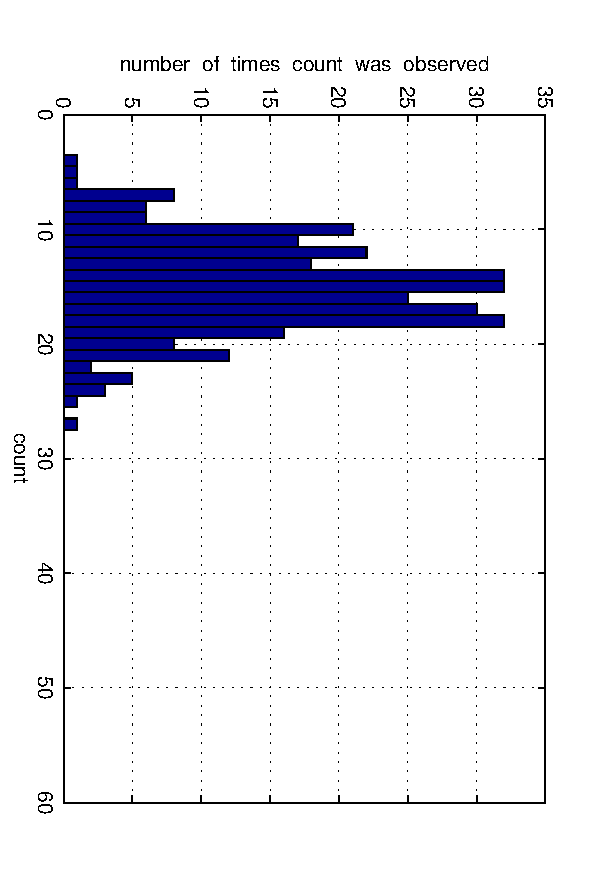
\includegraphics[scale=0.5, angle=90]{aPoissonExample.pdf}
\caption{Poisson Distribution Histogram}
\end{center}
\end{figure}

Load \texttt{hw2.mat} and run following code
\begin{verbatim}
hist(counts,1:50)
xlabel('count');ylabel('number of times count was observed');
hwplotprep
print -dpdf HW2Counts.pdf
\end{verbatim}

Replace \texttt{emptiness.pdf} with \texttt{HW2Counts.pdf} below.

\begin{figure}[H]
\begin{center}
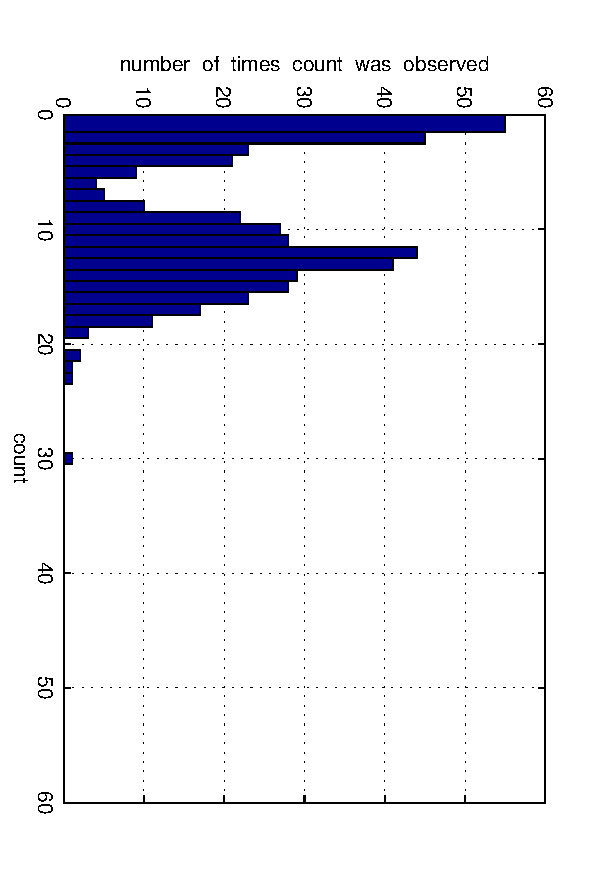
\includegraphics[scale=0.5, angle=90]{HW2Counts.pdf}
\caption{Homework 2 Counts Histogram.}
\end{center}
\end{figure}
Comment on the differences between the two histograms and a possible cause.

\textbf{Ans.} The first histogram is of a poisson distribution with mean $\lambda$ = 15. The second histogram is a combination of two distributions (poisson and normal). The first half can be explained by a Poission distribution with mean $\lambda <$ 5 and the second half of the histogram resembles a gaussian/normal distribution with a non-zero mean and variance.

\vspace{2mm}
\newproblem{1pt}
We will model a vector of counts $\xx$ as samples from a mixture of two Poisson distributions. The graphical model is simple
\begin{center}
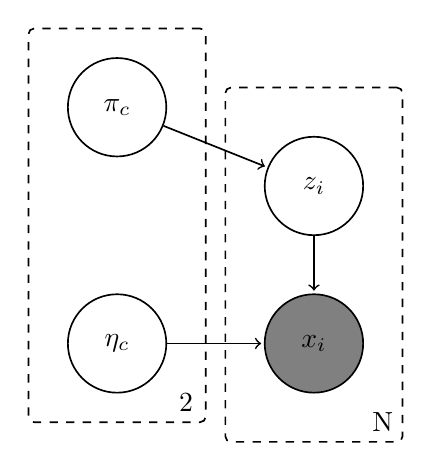
\begin{tikzpicture}[minimum size=1.25cm,->,shorten >=1pt,auto,node distance=1.75cm,semithick]
\tikzstyle{var}=[circle,fill=white,draw=black,text=black]
\tikzstyle{param}=[circle,fill=white,draw=black,text=black]
\node (Plate) [minimum width=2.25cm,minimum height=4.5cm,rounded corners=2pt,dashed,fill=none,draw=black] at ( 0.75,0) {};
\node (PlateLabel) [minimum size=0.5cm,anchor=south east] at  (Plate.south east) {N};
\node[var] (X1) at (0.75,1)  {$z_{i}$};
\node[var] (X2)  [fill=gray] at (0.75,-1) {$x_{i}$};
\node (Plate) [minimum width=2.25cm,minimum height=5cm,rounded corners=2pt,dashed,fill=none,draw=black] at ( -1.75,0.5) {};
\node (PlateLabel) [minimum size=0.5cm,anchor=south east] at  (Plate.south east) {2};
\node[param] (eta) at (-1.75,-1){$\eta_c$};
\node[param] (pi) at   (-1.75,2)  {$\pi_c$};
\path (X1) edge (X2);
\path (eta) edge (X2);
\path (pi) edge (X1);
\end{tikzpicture}
\end{center}
We will now derive and implement an EM algorithm for a mixture of two Poisson distributions.
\BEAS
p(z) &=& \begin{cases}
\pi_1, & z = 1\\
1 - \pi_2, & z = 2\\
\end{cases} \\
p(x|z) &=& h(x)\exp{\eta_z T(x) - A(\eta_z)}
\EEAS
Recall the structure of the an algorithm
\BEAS
E: q^{\textrm{new}} &=& \argmax_q  \sum_z q(\zz) \log p(\xx,\zz|\eta) - \sum_{\zz} q(\zz)\log q(\zz) \\
M: \eta^{\textrm new} &=& \argmax_\eta  \sum_{\zz} q^{\textrm{new}}(\zz) \log p(\xx,\zz|\eta) -\sum_{\zz} q^{\textrm{new}}(\zz)\log q^{\textrm{new}}(\zz)
\EEAS
In the case of exact EM $q(\zz) = p(\zz|\xx,\eta)$, further we note that computing $p(\zz|\xx,\eta)$ in the above model corresponds to marginalization in the graphical model
\begin{center}
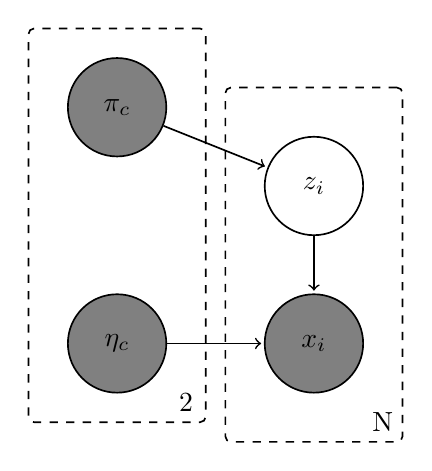
\begin{tikzpicture}[minimum size=1.25cm,->,shorten >=1pt,auto,node distance=1.75cm,semithick]
\tikzstyle{var}=[circle,fill=white,draw=black,text=black]
\tikzstyle{param}=[circle,fill=gray,draw=black,text=black]
\node (Plate) [minimum width=2.25cm,minimum height=4.5cm,rounded corners=2pt,dashed,fill=none,draw=black] at ( 0.75,0) {};
\node (PlateLabel) [minimum size=0.5cm,anchor=south east] at  (Plate.south east) {N};
\node[var] (X1) at (0.75,1)  {$z_{i}$};
\node[var] (X2)  [fill=gray] at (0.75,-1) {$x_{i}$};
\node (Plate) [minimum width=2.25cm,minimum height=5cm,rounded corners=2pt,dashed,fill=none,draw=black] at ( -1.75,0.5) {};
\node (PlateLabel) [minimum size=0.5cm,anchor=south east] at  (Plate.south east) {2};
\node[param] (eta) at (-1.75,-1){$\eta_c$};
\node[param] (pi) at   (-1.75,2)  {$\pi_c$};
\path (X1) edge (X2);
\path (eta) edge (X2);
\path (pi) edge (X1);
\end{tikzpicture}
\end{center}
Are $z_i$ conditionally independent given $\pi$ and $\xx$? \answer.
Describe reasoning behind your observation using Bayes ball paths. \answer.
\newproblem{1pt} We will now compute $q(z_i) = p(z_i | x_i,\eta)$ using Bayes rule
\[
q(z_i) = p(z_i | x_i,\eta) = \answer
\]
Note that you can use $\pi_{z_i}$ and $\eta_{z_i}$ notation to denote parameters of class $z_i$.
Write a Matlab function that computer $q(z_i)$
\begin{verbatim}
function qzi = computeQ(xi,etas,pis)
for c=1:2
    qzi(c) = log(...) %
end
qzi = exp(qzi - logsum(qzi));
\end{verbatim}
\newproblem{1pt} Recall M-step, where we eliminated portions of the objective that do not depend on $\eta$
\[
M: \eta^{\textrm new} = \argmax_\eta  \sum_{\zz} q^{\textrm{new}}(\zz) \log p(\xx,\zz|\eta)
\]
Show that the above expression is equal to
\[
M: \eta^{\textrm new} = \argmax_\eta  \sum_i q^{\textrm{new}}(z_i)\log p(x_i,\zz|\eta)
\]
We can say that
\[
p(\xx,\zz|\eta) = \prod_i p(x_i,z_i|\eta)
\]
because \answer.
Using the above equality and
\[
\sum_{\zz} q(\zz) f(z_i) = \sum_{z_i} q(z_i) f(z_i)
\]
we can rewrite the M-step update
\[
M: \eta^{\textrm new} = \argmax_\eta  \answer
\]
Take the derivative of the objective under the  $\argmax$ and set it to $0$ to obtain updates
\BEAS
\eta_1 &=& \answer\\
\eta_2 &=& \answer
\EEAS
write matlab code that implements M-step
\begin{verbatim}
function [etas,pis] = updateParameters(q,x)
pis = zeros(2,1);
for i=1:length(x)
    for c=1:2
        pis(c) = pis(c) + q(i,c);
    end
end
pis = pi/sum(pis);

for c=1:2
    for i=1:length(x)
        eta(c) = ...
    end
end
\end{verbatim}


\newproblem{2pt} Putting it all together,
\begin{verbatim}
function [eta,pi] = EMMoP(x)
etas = log(mean(x) + 0.0001*rand(2,1));
pis = 0.5*ones(2,1);

for it=1:MAXIT
    before = computeBound(q,x,etas,pis)
    for i=1:length(x)
        q(:,i) = computeQ(x(i),etas,pis);
    end
    after = computeBound(q,x,etas,pis);
    assert(after > before);
    before = after;
    [etas,pis] = updateParameters(q,x);
    after = computeBound(q,x,etas,pis);
    assert(after > before);
    bounds(it) = bound;
    plot(bounds);
    drawnow;
end

function bound = computeBound(q,x,etas,pis)
for i=1:length(x)
    for c=1:2
        bound = bound + q(c,i)*(etas(c)*x(i)-exp(etas(c))+log(pis(c)));
    end
end
for i=1:length(x)
    for c=1:2
        bound = bound - q(c,i)*log(q(c,i));
    end
end
\end{verbatim}
Load \texttt{hw2.mat} and run this code on \texttt{counts}. Report here resulting \texttt{eta,pi}
\begin{verbatim}
eta = ...
pi = ...
\end{verbatim}
\newproblem{1pt} Now we convert the above EM algorithm to K-means analog for Poisson distribution. Change function \texttt{computeQ} you implemented earlier to assign all probability to the most likely class, so each \texttt{qzi} should be binary.
\begin{verbatim}
function qzi = computeQ(xi,etas,pis)
for c=1:2
    qzi(c) = ... %
end
\end{verbatim}
Load \texttt{hw2.mat} and run \texttt{EMMoP} code on \texttt{x}. Report here resulting \texttt{etas,pis}
\begin{verbatim}
etas = ...
pis = ...
\end{verbatim}

\end{document}
